\section{Introduction}
The goal of this course was to teach a simulated robot arm to throw an object (in our case a blue cylinder) as far as it is possible within the given simulation. The simulation in this case ran in the Neurorobotics Platform (NRP) which utilizes the Robotic Simulator Gazebo and the spiking neural network simulator nest.\\%hier evtl. noch Weblinks zu NEST NRP GAZEBO 
The Experimental setup consisted of a table on which a HoLLiE robot arm and a blue cylinder were placed.
The initial setup can be seen in Fig. \ref{init_state}. For every iteration in the simulation the cylinder was placed at the exact same position. 
As the focus in this course was neurorobtics we used spiking neural networks as the basis of our machine learning approach.  
The goal was to find a suitable learning algorithm for a spiking neuronal network which could solve the task. We chose a reinforcement learning approach in combination with an evolutionary strategy to adjust the weights of the network.
For the simulation and design of the spiking neural network we used NRP including the SNN simulator NEST. For that the platform includes the following things:
 \begin{itemize}
\item a Gazebo environment and simulation
\item editors to create transfer functions to control the actors and get sensor data
\item a editor to create the neurons and synapsis of the network
\item a view output mechanism to monitor the simulation
\item a so called virtual coach configure and start simulations for the learning task.
\end{itemize} 
\begin{figure}[H]
	\centering
	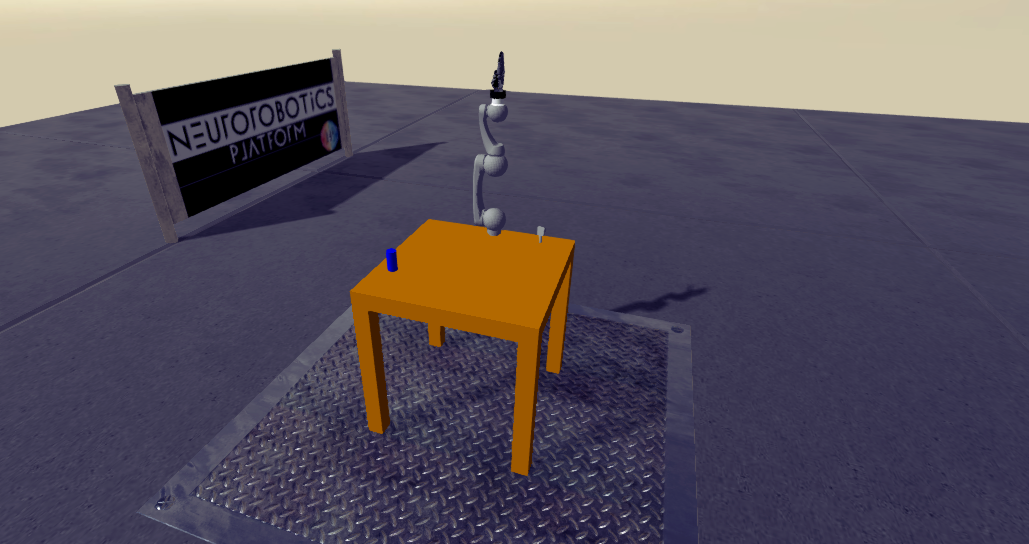
\includegraphics[width=2.2in]{img/init_state.png}
	\DeclareGraphicsExtensions.
	\caption{General task enviornment with inital state }
	\label{init_state}
\end{figure}

\section{Related Work}%muss noch korrigiert werden
As we use Reinforcment Learning and spiking neuronal networks we do here a short instruction to them.
\subsection{Reinforcment Learning}%muss noch korrigiert werden
Reinforcment Learning is based on the interaction of a agent (in our case the robot arm) with his environment (in our case Gazebo). To Learn, the agent get for every action in a state a reward(distance) - depending on if the action was good or not(far or short distance)- and a new state. If the action in the corresponded state got a high reward, then it's more likeliky that the actor uses the same action next time he is in this state again. To see a simple illustration of the whole learning process see Fig. \ref{re_base}
\begin{figure}[H]
	\centering
	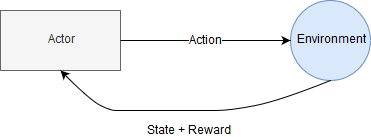
\includegraphics[width=2.2in]{img/re_base.png}
	\DeclareGraphicsExtensions.
	\caption{General illustration of reinforcement learning}
	\label{re_base}
\end{figure}

\subsection{Spiking Neuronal Networks}%muss noch korrigiert werden
Spiking neuronal networks is a variant of artifical neuronal (ANN) networks which are closer to the human brain as model then other ANN. In SNN the information isn't represented by the autoput value of a neuron, as spikes of a single neuron always looks the same, it's represented in the timing a neuron spikes. For example the information can be represented by the difference from the present spike to the last spike. To learn, there are, as in other ANN's weights which describes how much a output spike of a previous neuron influence the next neuron in order. To train the SNN u have to adept this weights, which is quiet difficult as there is no activation function like in standard ANNs. Compared to other ANNs in SNNs each neuron got a activation potential and every time this got exceeded the neuron spikes with a predefined spike.

\section{Throwing Challenge}
\subsection{Task}
The Task of this challenge was to teach the robot to throw the blue cylinder as far as possible. Since the robot arm is equipped with 6 different joints for the movement of the arm and several more for the hand, we simplified the movement. Firstly by combining the control of the hand joints into one grasping movement. Secondly by dividing the throwing movement into three seperate sub-movements which are:
 \begin{enumerate}
\item approaching the cylinder
\item grasping the cylinder
\item throwing the cylinder
\end{enumerate}
We chose to only learn the throwing movement with the help of SNNs because of several challenges which we examine in the following.

\subsection{Challenges}
\label{sec:challenges}
The biggest challenge in this task is that the simulation is non deterministic. Even when throwing the cylinder with fixed pre-defined movements of the robot arm, the results were not reproducible, which made it difficult to determine which movements were actually best for achieving a high distance. This also complicated the training of the SNN because we cannot reliably meassure the performance of the network.\\
Another problem was that the physical simulation of the interaction of the robot hand and the cylinder could lead to unintended bugs which lead to unrealistic high distances, that dominated in our training approaches.\\
In order to solve the challenge of non deterministic behaviour of the simulation a sollution would have been to run the experiment several times and choose the median of the achieved distances. But since it was not possible to speed up the simulation we decided to run the experimetn only once in order to decrease the time for training.\\




